%!TEX root = main.tex

\section{Prioritized Streaming String Transducers}  \label{sect:psst}
%\zhilin{Move from preliminary to here}

In this section, we introduce prioritized streaming string transducers (PSST), which extends prioritized finite-state automata (PFA) proposed in \cite{BM17}. We shall utilize PSST to model  the eager and greedy semantics of $\regexp$ as well as the behavior of $\replaceall$ functions with capturing groups and back references.
%based on which we model the semantics of $\regexp$ defined in Section~\ref{sec:prel} and design the decision procedure in Section~\ref{sec:decision}.

%\paragraph{Prioritized Finite-state automata.}
%
For a finite set $Q$, let $\overline{Q} = \bigcup_{n\in \Nat}\{ (q_1, \ldots, q_n) \mid \forall i \in [n], q_i \in Q \wedge \forall i,j \in[n], i \neq j \rightarrow q_i \neq q_j \}$. Intuitively, $\overline{Q}$ is the set of sequences of non-repetitive elements from $Q$. Note that the length of each sequence from $\overline{Q}$ is bounded by  $| Q |$. For a sequence $P = (q_0 \ldots q_n) \in \overline{Q}$ and  $q \in Q$, we write $q \in P$ if  $q = q_i$ for some $i \in [n]$. 


\begin{definition}[Prioritized Finite-state Automata]
  A \emph{prioritized finite-state automaton} (PFA) over a finite alphabet $\Sigma$ is a tuple $\pnfa=(Q, \Sigma, \delta, q_0, F)$ where $\delta \in Q
  \times \Sigma \rightarrow \overline{Q}$. The definition of $Q, q_0$ and $F$ is the same as ordinary FA.
  
A run of $\pnfa$ is the sequence $q_0 \sigma_1 q_1 \ldots \sigma_m q_m$, where $q_m \in F$ and for any $i \in [m], q_i \in \delta (q_{i - 1}, \sigma_i)$. For any two runs $p = q_0 \sigma_1 q_1 \ldots \sigma_m q_m$ and $p' =  q_0 \sigma_1 q_1' \ldots \sigma_m q_m'$ on $w = \sigma_1 \ldots \sigma_m$, we say that $p$ is of a higher priority over  $p'$ if $p \neq p'$, and for the smallest index $j$ with $q_j \neq q_j'$, $\delta (q_{j - 1}, \sigma_j) = \ldots q_j \ldots q_j' \ldots$.
  
An accepting run of $\pnfa$ on $w$ is the one with the highest priority. The language of $\pnfa$, denoted as $\Lang(\pnfa)$, is the set of
 strings on which $\pnfa$ has an accepting run.
\end{definition}

The priorities of PFA are used to model the eager and greedy semantics of $\regexp$, as we shall see in Section~\ref{construction:pnfa}.


%\paragraph{Prioritized streaming string transducers.}

We then introduce prioritized streaming string transducers, a new class of transducers that combine prioritized transducers \cite{BM17} %which combines the expressive power of 
and streaming string transducers \cite{AC10,AD11}.
  
\begin{definition}[Prioritized Streaming String Transducers]
A \emph{prioritized streaming string transducer} (PSST) is a tuple $\psst = (Q, \Sigma, X, \delta, E, q_0, F)$, where $Q$ a
finite set of states, $\Sigma$ is the input and output alphabet, and $X$ a finite set of variables, $\delta \in Q \times \Sigma \rightarrow \overline{Q}$, $E$ is a partial function from $Q \times \Sigma \times
  Q$ to $X \rightarrow (X \cup \Sigma)^{\ast}$, i.e. the set of assignments,
   $q_0 \in Q$ is the initial state, and $F$ is a partial function
  from $Q$ to $(X \cup \Sigma)^{\ast}$.

A run of $\psst$ is the sequence $q_0 \sigma_1 s_1 q_1 \ldots \sigma_m s_m q_m$, where $F (q_m)$ is defined and for each $i \in [m], q_i \in \delta (q_{i-1}, \sigma_i)$ and $s_i = E (q_{i - 1}, \sigma_i, q_i)$. For any two runs on $w = \sigma_1 \ldots \sigma_m$, denoted by $p = q_0 \sigma_1 s_1 \ldots \sigma_m s_m q_m$ and $p' = q_0 \sigma_1
  s_1' \ldots \sigma_m s_m' q_m'$, we say that $p$ is of a higher priority over
  $p'$ if $p \neq p'$ and, for the smallest index $j$ with $q_j \neq q_j'$,
  $\delta (q_{j - 1}, \sigma_j) = \ldots q_j \ldots q_j' \ldots$
  
  The accepting run of $\psst$ on an input $w$ is the run of the highest priority. The output of $\psst$ on $w$, denoted by $\psst(w)$, is defined as $\pi_m(F(q_m))$, where $\pi_0(x) = \varepsilon$ for each $x \in X$, and $\pi_{i}(x) = \pi_{i-1}(s_{i}(x))$ for every $1 \le i \le m$ and $x \in X$. Note that here we abuse the notation  $\pi_m(F(q_m))$ and $\pi_{i-1}(s_{i}(x))$ by taking a function $\pi$ from $X$ to $\Sigma^*$ as a function from $(X \cup \Sigma)^*$ to $\Sigma^*$, which maps each $\sigma \in \Sigma$ to $\sigma$ and each $x \in X$ to $\pi(x)$. If there is no accepting run of $\psst$ on $w$, then $\psst(w) = \bot$, namely, the output of $\psst$ on $w$ is undefined. The string relation defined by $\psst$, denoted by $\cR_\psst$,  is $\{(w, \psst(w)) \mid w \in \Sigma^\ast, \psst(w) \neq \bot\}$.
\end{definition}


\begin{example}
The PSST $\cT_{\sf nameReg}=(Q, \Sigma, X, \delta, E,  q_{0}, F$ mentioned in Section~\ref{sec:mot} is illustrated in Figure~\ref{fig-psst-exmp}, where $Q = \{q_0, \dots, q_{10}\}$, $X= \{x_1, x_2, x_3, x_4\}$ with $x_1, x_2, x_3$ recording the matches of the 1st, 2nd, 3rd capturing group, and $x_4$ recording the string after the replacements, $F(q_{10}) = x_4 x_2 \backslash {\rm s} x_1$ denotes the final output, and $\delta, E$ are illustrated by the edges, e.g. $\delta(q_4, \backslash\mbox{s}) = q_5q_{6}$ and $E(q_4, \backslash\mbox{s}, q_5)(x_2) = x_2 \backslash s$.  Note that the identity assignments, e.g. $E(q_4, \backslash\mbox{s}, q_5)(x') = x'$ for $x' \in \{x_1, x_3, x_4\}$, are omitted in Figure~\ref{fig-psst-exmp}, for readability. From $\delta(q_4, \backslash s) = q_5q_{6}$, we know that $q_5$ is prior to $q_6$. Therefore, whenever $\cT_{\sf nameReg}$ reads $\backslash$s at the state $q_4$,  it will choose to go the state $q_5$ greedily, unless this choice would lead to the nonacceptance (in this case, $q_6$ will be chosen). Moreover, the symbol $\ell$ is used therein to denote the current input letter scanned by $\cT_{\sf nameReg}$.
\begin{figure*}[ht]
\centering
%\rule{\linewidth}{0cm}
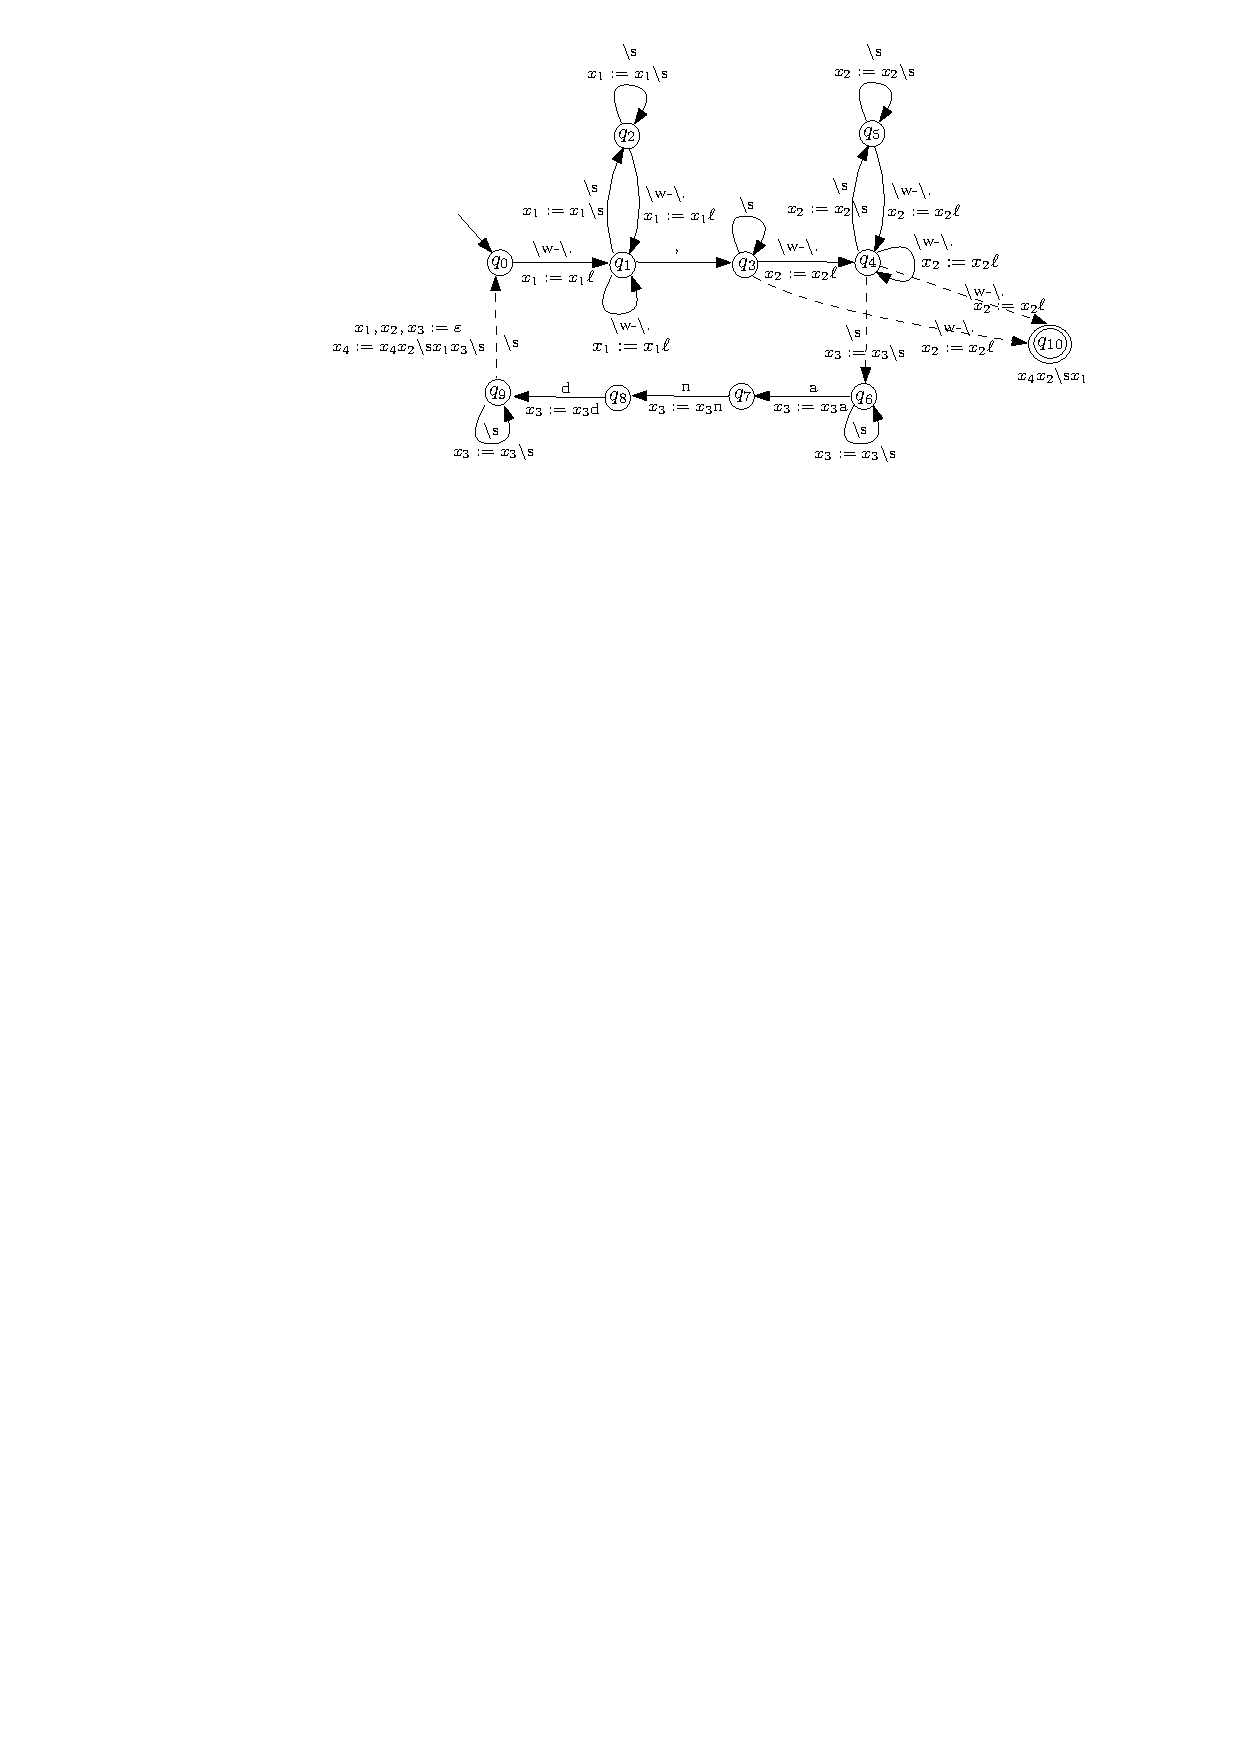
\includegraphics{psst-exmp.pdf}
\caption{The PSST $\cT_{\sf nameReg}$}
\label{fig-psst-exmp}
\end{figure*}
\end{example}

  
%  $\tmop{Out} (r) =
%  s_{\varepsilon} \circ s_1 \circ s_2 \ldots s_n \circ F (q_n)$ where
%  $s_{\varepsilon}$ is the empty substitution which maps all variables to
%  $\varepsilon$.
  
\begin{definition}[Pre-image]
For a string relation $R \subseteq \Sigma^* \times \Sigma^*$ and $L \subseteq \Sigma^*$, we define the \emph{pre-image} of $L$ under $R$ as $R^{-1}(L):=\{w \in \Sigma^* \mid \exists w'.\ w' \in L \mbox{ and } (w, w') \in R\}$. 
\end{definition}
 
\begin{theorem}[Pre-image of \PSST{}]
  \label{theorem:psst_preimage}
  Given a \PSST{} $\psst = (Q_T, \Sigma$, $X, \delta_T, E,  q_{0, T}, F_T)$ and an \FA{} $\Aut
  = (Q_A, \Sigma, \delta_A, q_{0, A}, F_A)$, we can compute an \FA{} $\cB = (Q_B,
  \Sigma, \delta_B, q_{0, B}, F_B)$ in exponential time  such that $\Lang(\cB) = \cR^{-1}_T(\Lang(\Aut))$.
\end{theorem}
 
\begin{proof}
Intuitively, $\cB$ simulates the run of $\psst$ on $w$, and, for each $x \in X$, records the set of state pairs $(p, q) \in Q_A \times Q_A$ such that starting from $p$, $\Aut$ can reach $q$ after reading the string stored in $x$. Moreover, $\cB$ also records all the states accessible from a run with higher priority to ensure the current run is the accepting one of $\psst$.

Formally, $Q_B = Q_T \times (\cP(Q_A \times Q_A ))^{X} \times \cP(Q_T)  $, $q_{0, B} = (q_{0, T}, \rho_{\varepsilon}, \emptyset)$ where $\rho_{\varepsilon} (x) = \{(q, q) \mid q \in Q\}$ for each $x \in X$, and $\delta_{B}$ comprises the tuples $((q, \rho, S), a, (q_i, \rho', S'))$ such that there exists $s \in \left((X \cup \Sigma\right)^*)^X$ satisfying
\begin{itemize}
\item $\delta_T (q, a) = (q_1 \ldots q_i \ldots q_m)$, 
\item $s = E(q,a,q_i)$.
\item $S' = \delta_T (S, a) \cup \{ q_1, \ldots, q_{i - 1} \}$, where $\delta_T(S,a) = \{q' \mid \exists q \in S, q' \in \delta_T(q,a)\}$.
\item and $\rho'$ is obtained from $\rho$ and $s$ as follows: for each $x \in X$, if $s(x) = \varepsilon$, then $\rho'(x) = \{(p, p) \mid p \in Q_A\}$, otherwise, let $s(x) = b_1 \cdots b_\ell$ with $b_i \in \Sigma \cup X$ for each $i \in [\ell]$, then $\rho'(x) = \theta_1 \circ \cdots \circ \theta_\ell$, where $\theta_i = \delta^{(b_i)}_A$ if $b_i \in \Sigma$, and $\theta_i = \rho(b_i)$ otherwise.
%
%$\rho'(x) = \theta_\ell$ such that $\theta_0 = \{(p,p) \mid p \in Q_A\}$, and for each $i \in [\ell]$, if $b_i \in \Sigma$, then $\theta_i = \{(p, p') \mid (p, p'') \in \theta_{i-1}, (p'', b_i, p') \in \delta_A \mbox{ for some } p''\}$, otherwise, $\theta_i = \theta_{i-1} \cdot \rho(x)$. 
\end{itemize}

Moreover, $F_B$ is the set of states $(q, \rho, S) \in Q_B$ such that
\begin{enumerate}
  \item $F_T (q)$ is defined,
%
  \item for any $q' \in S$, $F_T (q')$ is not defined,
  %
  \item if $F_T(q) = \varepsilon$, then $q_{0, A}  \in F_A$, otherwise, 
let $F_T(q) = b_1 \cdots b_\ell$ with $b_i \in \Sigma \cup X$ for each $i \in [\ell]$, then $(\theta_1 \circ \cdots \circ \theta_\ell) \cap (\{q_{0,A}\} \times F_A) \neq \emptyset$, where for each $i \in [\ell]$, if $b_i \in \Sigma$, then $\theta_i = \delta^{(b_i)}_A$, otherwise, $\theta_i = \rho(b_i)$.
\end{enumerate}
\end{proof}

Note that the above construction  does not utilize the so-called \tmtextit{copyless} property \cite{AC10,AD11},
  thus it works for general, or \tmtextit{copyful} \PSST{} \cite{FR17}.

% Note that in the definition of \NSST, there is no \emph{copyless} restriction.



